
\documentclass[tikz,border=2]{standalone}
\usetikzlibrary{shadows,arrows,shapes,positioning,calc,backgrounds,fit}
\usepackage{amssymb}
\usepackage{array}
\usepackage{colortbl}
\pdfpageattr {/Group << /S /Transparency /I true /CS /DeviceRGB>>}
\newcommand{\lens}[7]{ % ux,uy,vx,vy,in,out,color
\path[fill=#7,out=#5,in=#6] (#1,#2) -- (#3,#4);
}
\newcommand{\lensarrow}[7]{ % ux,uy,vx,vy,in,out,arrowwidth
\draw[-{Latex[width=#7},out=#5,in=#6] (#1,#2) -- (#3,#4);
}

% custom colors
\definecolor{c0}{HTML}{D16103}
\definecolor{c1}{HTML}{52854C}
\definecolor{c2}{HTML}{293352}

\begin{document}
\begin{tikzpicture}
% Nodes
\node[draw,draw=none] (0) at (11.932657459639922,5.100226691630441) {\includegraphics[width=.5cm]{../data/home.png}};
\node[draw,draw=none] (1) at (0.5887727289367153,14.93520000000043) {\includegraphics[width=.5cm]{../data/home.png}};
\node[draw,draw=none] (2) at (4.682686650024401,11.557495278173228) {\includegraphics[width=.5cm]{../data/home.png}};
\node[draw,draw=none] (3) at (12.364227307689976,0.8016206180622195) {\includegraphics[width=.5cm]{../data/other.png}};
\node[draw,draw=none] (4) at (3.763024447259322,3.1475654251311953) {\includegraphics[width=.5cm]{../data/work.png}};
\node[draw,draw=none] (5) at (3.570806866942973,4.353272869948366) {\includegraphics[width=.5cm]{../data/work.png}};
\node[draw,draw=none] (6) at (7.400135554514235,0.7111999999995692) {\includegraphics[width=.5cm]{../data/work.png}};

% Edges
\draw[,dashed] (0) edge[,line width=1.5mm,>=latex,opacity=0.7,color=c0,out=-164.9,in=-4.9,->] (5);
\draw[,dashed] (5) edge[,line width=1.5mm,>=latex,opacity=0.7,color=c0,out=-31.99,in=168.01,->] (3);
\draw[,dashed] (3) edge[,line width=1.5mm,>=latex,opacity=0.7,color=c0,out=85.73,in=-74.27,->] (0);
\draw[,dash dot dot] (1) edge[,line width=1.5mm,>=latex,opacity=0.7,color=c1,out=-64.93,in=95.07,->] (4);
\draw[,dash dot dot] (4) edge[,line width=1.5mm,>=latex,opacity=0.7,color=c1,out=115.07,in=-84.93,->] (1);
\draw[,dash dot] (2) edge[,line width=1.5mm,>=latex,opacity=0.7,color=c2,out=-85.93,in=114.07,->] (6);
\draw[,dash dot] (6) edge[,line width=1.5mm,>=latex,opacity=0.7,color=c2,out=94.07,in=-65.93,->] (2);

\begin{pgfonlayer}{background}
\node[anchor=south west] {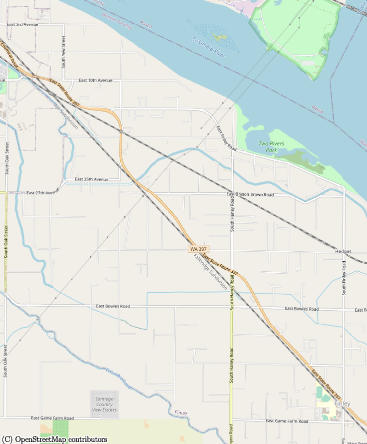
\includegraphics[width=12.953000036626692cm]{activities_base}};
\end{pgfonlayer}

\end{tikzpicture}
\end{document}
